\documentclass[tikz,border=4pt]{standalone}
\usepackage{ctex}
\usepackage{pgfplots}
\pgfplotsset{compat=1.18}
\begin{document}
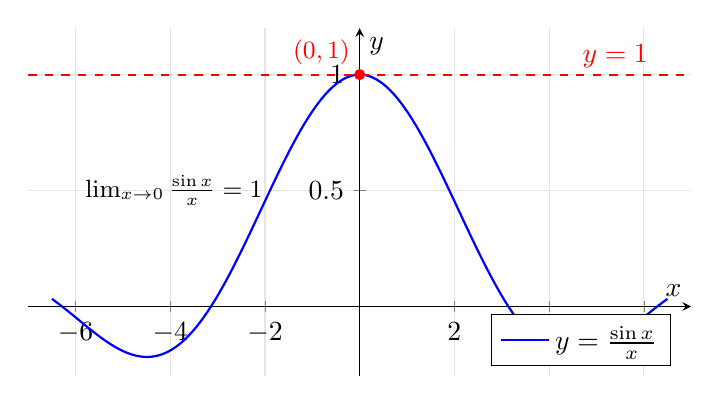
\begin{tikzpicture}
\begin{axis}[
    axis lines=middle, width=10cm, height=6cm,
    xmin=-7, xmax=7, ymin=-0.3, ymax=1.2,
    xlabel={$x$}, ylabel={$y$},
    samples=300, grid=both, grid style={gray!20},
    legend pos=south east,
]
\addplot[blue, thick, domain=-6.5:-0.01] {sin(deg(x))/x};
\addplot[blue, thick, domain=0.01:6.5] {sin(deg(x))/x};
\addlegendentry{$y=\frac{\sin x}{x}$}
\draw[red, thick, dashed] (axis cs:-7,1) -- (axis cs:7,1);
\node[red, anchor=west] at (axis cs:4.5, 1.08) {$y=1$};
\fill[red] (axis cs:0,1) circle (2pt);
\node[anchor=south east, red] at (axis cs:0,1) {\small $(0,1)$};
\node[anchor=west] at (axis cs:-6, 0.5) {\small $\lim_{x\to 0}\frac{\sin x}{x}=1$};
\end{axis}
\end{tikzpicture}
\end{document}
